% Options for packages loaded elsewhere
\PassOptionsToPackage{unicode}{hyperref}
\PassOptionsToPackage{hyphens}{url}
\PassOptionsToPackage{dvipsnames,svgnames,x11names}{xcolor}
%
\documentclass[
  letterpaper,
  DIV=11,
  numbers=noendperiod]{scrreprt}

\usepackage{amsmath,amssymb}
\usepackage{lmodern}
\usepackage{iftex}
\ifPDFTeX
  \usepackage[T1]{fontenc}
  \usepackage[utf8]{inputenc}
  \usepackage{textcomp} % provide euro and other symbols
\else % if luatex or xetex
  \usepackage{unicode-math}
  \defaultfontfeatures{Scale=MatchLowercase}
  \defaultfontfeatures[\rmfamily]{Ligatures=TeX,Scale=1}
\fi
% Use upquote if available, for straight quotes in verbatim environments
\IfFileExists{upquote.sty}{\usepackage{upquote}}{}
\IfFileExists{microtype.sty}{% use microtype if available
  \usepackage[]{microtype}
  \UseMicrotypeSet[protrusion]{basicmath} % disable protrusion for tt fonts
}{}
\makeatletter
\@ifundefined{KOMAClassName}{% if non-KOMA class
  \IfFileExists{parskip.sty}{%
    \usepackage{parskip}
  }{% else
    \setlength{\parindent}{0pt}
    \setlength{\parskip}{6pt plus 2pt minus 1pt}}
}{% if KOMA class
  \KOMAoptions{parskip=half}}
\makeatother
\usepackage{xcolor}
\setlength{\emergencystretch}{3em} % prevent overfull lines
\setcounter{secnumdepth}{5}
% Make \paragraph and \subparagraph free-standing
\ifx\paragraph\undefined\else
  \let\oldparagraph\paragraph
  \renewcommand{\paragraph}[1]{\oldparagraph{#1}\mbox{}}
\fi
\ifx\subparagraph\undefined\else
  \let\oldsubparagraph\subparagraph
  \renewcommand{\subparagraph}[1]{\oldsubparagraph{#1}\mbox{}}
\fi


\providecommand{\tightlist}{%
  \setlength{\itemsep}{0pt}\setlength{\parskip}{0pt}}\usepackage{longtable,booktabs,array}
\usepackage{calc} % for calculating minipage widths
% Correct order of tables after \paragraph or \subparagraph
\usepackage{etoolbox}
\makeatletter
\patchcmd\longtable{\par}{\if@noskipsec\mbox{}\fi\par}{}{}
\makeatother
% Allow footnotes in longtable head/foot
\IfFileExists{footnotehyper.sty}{\usepackage{footnotehyper}}{\usepackage{footnote}}
\makesavenoteenv{longtable}
\usepackage{graphicx}
\makeatletter
\def\maxwidth{\ifdim\Gin@nat@width>\linewidth\linewidth\else\Gin@nat@width\fi}
\def\maxheight{\ifdim\Gin@nat@height>\textheight\textheight\else\Gin@nat@height\fi}
\makeatother
% Scale images if necessary, so that they will not overflow the page
% margins by default, and it is still possible to overwrite the defaults
% using explicit options in \includegraphics[width, height, ...]{}
\setkeys{Gin}{width=\maxwidth,height=\maxheight,keepaspectratio}
% Set default figure placement to htbp
\makeatletter
\def\fps@figure{htbp}
\makeatother
\newlength{\cslhangindent}
\setlength{\cslhangindent}{1.5em}
\newlength{\csllabelwidth}
\setlength{\csllabelwidth}{3em}
\newlength{\cslentryspacingunit} % times entry-spacing
\setlength{\cslentryspacingunit}{\parskip}
\newenvironment{CSLReferences}[2] % #1 hanging-ident, #2 entry spacing
 {% don't indent paragraphs
  \setlength{\parindent}{0pt}
  % turn on hanging indent if param 1 is 1
  \ifodd #1
  \let\oldpar\par
  \def\par{\hangindent=\cslhangindent\oldpar}
  \fi
  % set entry spacing
  \setlength{\parskip}{#2\cslentryspacingunit}
 }%
 {}
\usepackage{calc}
\newcommand{\CSLBlock}[1]{#1\hfill\break}
\newcommand{\CSLLeftMargin}[1]{\parbox[t]{\csllabelwidth}{#1}}
\newcommand{\CSLRightInline}[1]{\parbox[t]{\linewidth - \csllabelwidth}{#1}\break}
\newcommand{\CSLIndent}[1]{\hspace{\cslhangindent}#1}

\KOMAoption{captions}{tableheading}
\makeatletter
\@ifpackageloaded{tcolorbox}{}{\usepackage[many]{tcolorbox}}
\@ifpackageloaded{fontawesome5}{}{\usepackage{fontawesome5}}
\definecolor{quarto-callout-color}{HTML}{909090}
\definecolor{quarto-callout-note-color}{HTML}{0758E5}
\definecolor{quarto-callout-important-color}{HTML}{CC1914}
\definecolor{quarto-callout-warning-color}{HTML}{EB9113}
\definecolor{quarto-callout-tip-color}{HTML}{00A047}
\definecolor{quarto-callout-caution-color}{HTML}{FC5300}
\definecolor{quarto-callout-color-frame}{HTML}{acacac}
\definecolor{quarto-callout-note-color-frame}{HTML}{4582ec}
\definecolor{quarto-callout-important-color-frame}{HTML}{d9534f}
\definecolor{quarto-callout-warning-color-frame}{HTML}{f0ad4e}
\definecolor{quarto-callout-tip-color-frame}{HTML}{02b875}
\definecolor{quarto-callout-caution-color-frame}{HTML}{fd7e14}
\makeatother
\makeatletter
\makeatother
\makeatletter
\@ifpackageloaded{bookmark}{}{\usepackage{bookmark}}
\makeatother
\makeatletter
\@ifpackageloaded{caption}{}{\usepackage{caption}}
\AtBeginDocument{%
\ifdefined\contentsname
  \renewcommand*\contentsname{Table of contents}
\else
  \newcommand\contentsname{Table of contents}
\fi
\ifdefined\listfigurename
  \renewcommand*\listfigurename{List of Figures}
\else
  \newcommand\listfigurename{List of Figures}
\fi
\ifdefined\listtablename
  \renewcommand*\listtablename{List of Tables}
\else
  \newcommand\listtablename{List of Tables}
\fi
\ifdefined\figurename
  \renewcommand*\figurename{Figure}
\else
  \newcommand\figurename{Figure}
\fi
\ifdefined\tablename
  \renewcommand*\tablename{Table}
\else
  \newcommand\tablename{Table}
\fi
}
\@ifpackageloaded{float}{}{\usepackage{float}}
\floatstyle{ruled}
\@ifundefined{c@chapter}{\newfloat{codelisting}{h}{lop}}{\newfloat{codelisting}{h}{lop}[chapter]}
\floatname{codelisting}{Listing}
\newcommand*\listoflistings{\listof{codelisting}{List of Listings}}
\makeatother
\makeatletter
\@ifpackageloaded{caption}{}{\usepackage{caption}}
\@ifpackageloaded{subcaption}{}{\usepackage{subcaption}}
\makeatother
\makeatletter
\@ifpackageloaded{tcolorbox}{}{\usepackage[many]{tcolorbox}}
\makeatother
\makeatletter
\@ifundefined{shadecolor}{\definecolor{shadecolor}{rgb}{.97, .97, .97}}
\makeatother
\makeatletter
\makeatother
\ifLuaTeX
  \usepackage{selnolig}  % disable illegal ligatures
\fi
\IfFileExists{bookmark.sty}{\usepackage{bookmark}}{\usepackage{hyperref}}
\IfFileExists{xurl.sty}{\usepackage{xurl}}{} % add URL line breaks if available
\urlstyle{same} % disable monospaced font for URLs
\hypersetup{
  pdftitle={Data Science for Public Health},
  pdfauthor={Hélène Langet; Samwel Lwambura; Fenella Beynon; Silvia Cicconi},
  colorlinks=true,
  linkcolor={blue},
  filecolor={Maroon},
  citecolor={Blue},
  urlcolor={Blue},
  pdfcreator={LaTeX via pandoc}}

\title{Data Science for Public Health}
\usepackage{etoolbox}
\makeatletter
\providecommand{\subtitle}[1]{% add subtitle to \maketitle
  \apptocmd{\@title}{\par {\large #1 \par}}{}{}
}
\makeatother
\subtitle{Test}
\author{Hélène Langet \and Samwel Lwambura \and Fenella
Beynon \and Silvia Cicconi}
\date{2022-09-23T00:00:00+03:00}

\begin{document}
\maketitle
\ifdefined\Shaded\renewenvironment{Shaded}{\begin{tcolorbox}[interior hidden, enhanced, sharp corners, boxrule=0pt, breakable, frame hidden, borderline west={3pt}{0pt}{shadecolor}]}{\end{tcolorbox}}\fi

\renewcommand*\contentsname{Table of contents}
{
\hypersetup{linkcolor=}
\setcounter{tocdepth}{2}
\tableofcontents
}
\bookmarksetup{startatroot}

\hypertarget{preface}{%
\chapter*{Preface}\label{preface}}
\addcontentsline{toc}{chapter}{Preface}

\hypertarget{introduction}{%
\section*{Introduction}\label{introduction}}
\addcontentsline{toc}{section}{Introduction}

Data science and artificial intelligence have the potential to generate
fundamentally new insights on global health policies in Africa, but the
full realization of this potential depends on the availability of a
critical mass of highly trained health data scientists on the continent.

This electronic book was created by Hélène Langet, Fenella Beynon,
Fabian Schär, Silvia Cicconi and Gillian Levine from the
\href{https://www.swisstph.ch}{Swiss Tropical \& Public Health Institute
(Swiss TPH)} and Samwel Lwambura (IHI) from the
\href{https://ihi.or.tz/}{Ifakara Health Institute (IHI)} to accompany
the \textbf{Data Science for Public Health} workshop which will be held
in Dar-es-Salaam from Monday,September 26th to Wednesday, September 28th
2022.

The goal of this workshop is to enable researchers from the Ifakara
Health Institute (IHI) to strengthen their expertise in the area and to
lay the foundations for the development of a data science curriculum
that is adapted to IHI's needs.

This work is the product of interdisciplinary discussions with Abdallah
Mkopi, Grace Mhalu, Robert Moshiro from IHI and feedback from Hajirani
Msuya and Martine Masonda, the first group to use these notebooks.

\hypertarget{license}{%
\section*{License}\label{license}}
\addcontentsline{toc}{section}{License}

\includegraphics{https://i.creativecommons.org/l/by/4.0/88x31.png} This
book is licensed under a
\href{https://creativecommons.org/licenses/by/4.0/}{Attribution 4.0
International (CC BY 4.0)}.

You are free to:

\begin{itemize}
\tightlist
\item
  Share --- copy and redistribute the material in any medium or format
\item
  Adapt --- remix, transform, and build upon the material for any
  purpose, even commercially.
\end{itemize}

Under the following terms:

\begin{itemize}
\tightlist
\item
  Attribution --- You must give appropriate credit, provide a link to
  the license, and indicate if changes were made. You may do so in any
  reasonable manner, but not in any way that suggests the licensor
  endorses you or your use.
\item
  No additional restrictions --- You may not apply legal terms or
  technological measures that legally restrict others from doing
  anything the license permits.
\end{itemize}

\hypertarget{update-history}{%
\section*{Update History}\label{update-history}}
\addcontentsline{toc}{section}{Update History}

\begin{itemize}
\tightlist
\item
  September 25, 2022: First edition.
\end{itemize}

\hypertarget{acknowledgement}{%
\section*{Acknowledgement}\label{acknowledgement}}
\addcontentsline{toc}{section}{Acknowledgement}

This work was funded by the
\href{https://www.swisstph.ch/en/research/leading-house-africa/}{Leading
House Africa (LHA)} which promotes and fosters bilateral collaboration
with partner institutions in Africa.

\bookmarksetup{startatroot}

\hypertarget{about-the-workshop}{%
\chapter{About the workshop}\label{about-the-workshop}}

{🗓️} September 26-28, 2022\\
{🕘} 09:00 - 17:00\\
{🌇} Dar-es-Salaam, Tanzania

This workshop targets public health researchers and aims to accompany
them in their journey towards Data Science.

The workshop takes place at \textbf{Protea Hotel Dar es Salaam
Courtyard} on Seaview Ocean Road. The conference room is \textbf{Nelson
Hall}.

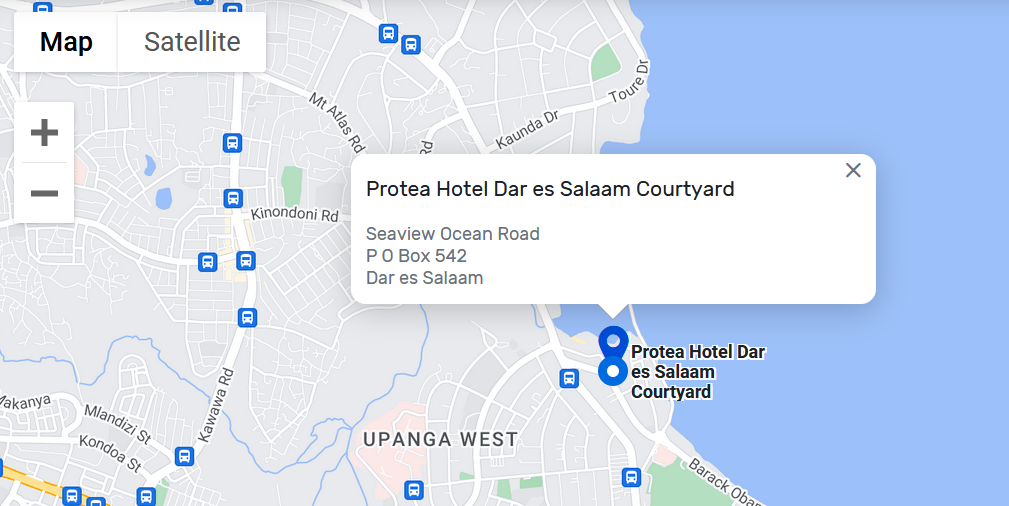
\includegraphics{./images/paste-67B4C38F.png}

\hypertarget{learning-objectives}{%
\section{Learning objectives}\label{learning-objectives}}

There are two complementary aspects of moving into data science:

\begin{enumerate}
\def\labelenumi{\arabic{enumi}.}
\tightlist
\item
  a \textbf{mindset} about how scientists think and collaborate about
  data, and
\item
  a \textbf{skillset} which is composed of an ecosystem of tools (mostly
  open-source) and practices.
\end{enumerate}

Upon completing the workshop, participants will have gained:

\begin{itemize}
\tightlist
\item
  exposure to data science approach, tools and collaborative practices
\item
  hands-on experience on how to interface between Stata and R, learned
  the basics of working with data in R/RStudio, and how to incrementally
  incorporate R into your existing data analysis workflows in Stata. The
  idea is not to replace everything you do in Stata into R but that you
  can continue your learning after this workshop at your own pace.
\end{itemize}

\hypertarget{is-this-workshop-for-me}{%
\section{Is this workshop for me?}\label{is-this-workshop-for-me}}

This workshop is relevant for individuals who answer yes to the
following questions:

\begin{itemize}
\tightlist
\item[$\square$]
  Do you who want to develop data science projects in public health?
\item[$\square$]
  Do you wants to learn more about how open and reproducible science
  approaches can be used in your daily practice?
\item[$\square$]
  Are you a Stata user (or any other data analysis language) who would
  like to expand your data analysis skillset with R?
\item[$\square$]
  Do you want to bridge analyses between data analysis tools (Stata, R
  or Python) and to more easily collaborate with other researchers who
  use another of these tools?
\end{itemize}

\hypertarget{to-do-before-the-workshop}{%
\section{To do before the workshop}\label{to-do-before-the-workshop}}

\begin{enumerate}
\def\labelenumi{\arabic{enumi}.}
\item
  Fill out the online
  \href{https://timicodktest.smartforest.de/-/single/cac06e76b3e163e655e49626f8129de8f55a8035ced54f15bc4c6cf527dba8a7?st=DnBRz677PIYh33ML0rE1amWzyhCIYPGFQnmZ6AAou8nJFyikWN6nLM5i3G4I0YZN}{pre-workshop
  questionnaire}
\item
  If you have not it yet, please go through the following five steps
  (about 30 minutes).

  \begin{enumerate}
  \def\labelenumii{\alph{enumii}.}
  \item
    Install R (\textbf{?@sec-R-installation})
  \item
    Install and setup RStudio Desktop
    (Section~\ref{sec-RStudio-installation})
  \item
    Install Quarto (Section~\ref{sec-Quarto-installation})
  \item
    Install the rmarkdown R package
    (Section~\ref{sec-rmarkdown-installation})
  \item
    Create a GitHub account (\textbf{?@sec-GitHub-account-creation})
  \item
    Install GitHub Desktop
    (Section~\ref{sec-GitHub-Desktop-installation})
  \end{enumerate}
\end{enumerate}

\begin{tcolorbox}[enhanced jigsaw, bottomtitle=1mm, title=\textcolor{quarto-callout-note-color}{\faInfo}\hspace{0.5em}{Note}, toptitle=1mm, toprule=.15mm, breakable, colframe=quarto-callout-note-color-frame, coltitle=black, rightrule=.15mm, arc=.35mm, left=2mm, opacitybacktitle=0.6, colback=white, colbacktitle=quarto-callout-note-color!10!white, bottomrule=.15mm, opacityback=0, titlerule=0mm, leftrule=.75mm]

\begin{itemize}
\tightlist
\item
  All software used in this workshop are free.
\item
  If you have any difficulties with the installation, support can be
  provided on the first day of the workshop before the first session or
  during breaks.
\end{itemize}

\end{tcolorbox}

\begin{tcolorbox}[enhanced jigsaw, bottomtitle=1mm, title=\textcolor{quarto-callout-important-color}{\faExclamation}\hspace{0.5em}{Important}, toptitle=1mm, toprule=.15mm, breakable, colframe=quarto-callout-important-color-frame, coltitle=black, rightrule=.15mm, arc=.35mm, left=2mm, opacitybacktitle=0.6, colback=white, colbacktitle=quarto-callout-important-color!10!white, bottomrule=.15mm, opacityback=0, titlerule=0mm, leftrule=.75mm]
For those who have already been introduced to Git, R/RStudio and
RMarkdown, note that you need to additionally install Quarto for this
workshop.
\end{tcolorbox}

\hypertarget{schedule}{%
\section{Schedule}\label{schedule}}

\hypertarget{day-1}{%
\subsection{Day 1}\label{day-1}}

\hypertarget{tbl-day1-schedule}{}
\begin{longtable}[]{@{}
  >{\centering\arraybackslash}p{(\columnwidth - 2\tabcolsep) * \real{0.2222}}
  >{\raggedright\arraybackslash}p{(\columnwidth - 2\tabcolsep) * \real{0.6528}}@{}}
\caption{\label{tbl-day1-schedule}Schedule Day 1}\tabularnewline
\toprule()
\begin{minipage}[b]{\linewidth}\centering
Time
\end{minipage} & \begin{minipage}[b]{\linewidth}\raggedright
Session
\end{minipage} \\
\midrule()
\endfirsthead
\toprule()
\begin{minipage}[b]{\linewidth}\centering
Time
\end{minipage} & \begin{minipage}[b]{\linewidth}\raggedright
Session
\end{minipage} \\
\midrule()
\endhead
08.30 - 09.00 & \begin{minipage}[t]{\linewidth}\raggedright
Welcome\\
Support for software installation\strut
\end{minipage} \\
09.00 - 09.15 & \begin{minipage}[t]{\linewidth}\raggedright
Introduction to data science tools\\
Overview of objectives for Day 1\strut
\end{minipage} \\
09.15 - 10.15 & Version control with Git \\
10.15 - 10.45 & {🍵} {☕} Break \\
10.45 -11.45 & Introduction to dynamic documents and Quarto \\
11.45 - 12.15 & Use Quarto with Stata \\
12.15 - 13.15 & {🍴} Lunch break \\
13.15 - 14.00 & Import external data \\
14.00 - 15.00 & Manipulate data \\
15.00 - 15.30 & {🍵} {☕} Break \\
15.30 - 16.15 & Visualise data \\
16.15 - 17.00 & Share code and collaborate with Git \\
\bottomrule()
\end{longtable}

\hypertarget{day-2}{%
\subsection{Day 2}\label{day-2}}

\hypertarget{tbl-day2-schedule}{}
\begin{longtable}[]{@{}
  >{\centering\arraybackslash}p{(\columnwidth - 2\tabcolsep) * \real{0.1702}}
  >{\raggedright\arraybackslash}p{(\columnwidth - 2\tabcolsep) * \real{0.8298}}@{}}
\caption{\label{tbl-day2-schedule}Schedule Day 2}\tabularnewline
\toprule()
\begin{minipage}[b]{\linewidth}\centering
Time
\end{minipage} & \begin{minipage}[b]{\linewidth}\raggedright
Session (all)
\end{minipage} \\
\midrule()
\endfirsthead
\toprule()
\begin{minipage}[b]{\linewidth}\centering
Time
\end{minipage} & \begin{minipage}[b]{\linewidth}\raggedright
Session (all)
\end{minipage} \\
\midrule()
\endhead
08.30 - 09.00 & Welcome \\
09.00 - 09.20 & \begin{minipage}[t]{\linewidth}\raggedright
Introduction to Data Science for Public Health\\
Overview of objectives for Day 2\strut
\end{minipage} \\
09.20 - 10.15 & Discussion on concepts related to to public health data
for decision-making \\
10.15 - 10.45 & {🍵} {☕} Break \\
10:45-12:15 & Malaria practical \#1 \\
12.15- 13.15 & {🍴} Lunch break \\
13.15- 13.30 & Prepare presentation of data findings \\
13.30 - 14.00 & Present and discuss data findings \\
14.00 - 14.30 & Interdisciplinary discussion on malaria, dataset,
uncertainties, challenges \\
14.00 - 14.30 & Malaria practical \#2 \\
15.00 - 15.30 & {🍵} {☕} Break \\
15.30 - 16.15 & Malaria practical \#2 \\
16.15 - 16.30 & Prepare presentation of data findings \\
16.30 - 17.00 & Present and discuss data findings \\
\bottomrule()
\end{longtable}

\hypertarget{day-3}{%
\subsection{Day 3}\label{day-3}}

\hypertarget{tbl-day3-schedule}{}
\begin{longtable}[]{@{}
  >{\centering\arraybackslash}p{(\columnwidth - 2\tabcolsep) * \real{0.1905}}
  >{\raggedright\arraybackslash}p{(\columnwidth - 2\tabcolsep) * \real{0.8095}}@{}}
\caption{\label{tbl-day3-schedule}Schedule Day 3}\tabularnewline
\toprule()
\begin{minipage}[b]{\linewidth}\centering
Time
\end{minipage} & \begin{minipage}[b]{\linewidth}\raggedright
Session (all)
\end{minipage} \\
\midrule()
\endfirsthead
\toprule()
\begin{minipage}[b]{\linewidth}\centering
Time
\end{minipage} & \begin{minipage}[b]{\linewidth}\raggedright
Session (all)
\end{minipage} \\
\midrule()
\endhead
08.30 - 09.00 & Welcome \\
09.00 - 09.20 & Interdisciplinary introduction to big data and machine
Learning

Overview of objectives for Day 3 \\
09.20 - 10.15 & Discussion on secondary data sources

(Public Datasets, e.g.~DHS, Facebook, facilities, etc)

Benefits and drawbacks between primary and secondary data sources \\
10.15 - 10.45 & {🍵} {☕} Break \\
10.45 - 12.15 & \begin{minipage}[t]{\linewidth}\raggedright
{[}Analysis stream{]} Introduction to machine learning\\
{[}Interpretation stream{]} Critically discuss data
surveys/reports\strut
\end{minipage} \\
12:15-13:15 & {🍴} Lunch break \\
13:15-13:45 & Speed talks - research presentations \\
13:45-15.00 & \begin{minipage}[t]{\linewidth}\raggedright
{[}Analysis stream{]} Data practical\\
{[}Interpretation stream{]} Critically discuss data
surveys/reports\strut
\end{minipage} \\
15.00 - 15.30 & {🍵} {☕} Break \\
15:30-16:00 & Feedback on findings from practicals \\
\begin{minipage}[t]{\linewidth}\centering
16:00-16:30\\
\strut
\end{minipage} & Feedback on workshop - Wrap-up \\
\bottomrule()
\end{longtable}

\hypertarget{to-do-after-the-workshop}{%
\section{To do after the workshop}\label{to-do-after-the-workshop}}

\begin{enumerate}
\def\labelenumi{\arabic{enumi}.}
\tightlist
\item
  Fill out the online post-workshop questionnaire.
\item
  This material will stay online, do not hesitate to refer to it if
  needed.
\end{enumerate}

\bookmarksetup{startatroot}

\hypertarget{references}{%
\chapter*{References}\label{references}}
\addcontentsline{toc}{chapter}{References}

\hypertarget{refs}{}
\begin{CSLReferences}{0}{0}
\end{CSLReferences}

\appendix
\addcontentsline{toc}{part}{Appendices}

\hypertarget{r-installations}{%
\chapter{R installations}\label{r-installations}}

\textbf{R} is a programming language for statistical computing and
graphics. It is one of main programming language used for data science
(with other programming languages such as Python and Julia).

\hypertarget{step-1}{%
\subsubsection{Step 1}\label{step-1}}

You can download R from the
\href{https://cran.r-project.org/mirrors.html}{Comprehensive R Archive
Network (CRAN)} which is a network of servers around the world that
store identical up-to-date versions of code and documentation for R.


\includegraphics{./images/paste-13103C13.png}

Scroll down the page to locate the mirror that is the closest to your
geographic location and click on its URL.

\begin{tcolorbox}[enhanced jigsaw, bottomtitle=1mm, title=\textcolor{quarto-callout-tip-color}{\faLightbulb}\hspace{0.5em}{Tip}, toptitle=1mm, toprule=.15mm, breakable, colframe=quarto-callout-tip-color-frame, coltitle=black, rightrule=.15mm, arc=.35mm, left=2mm, opacitybacktitle=0.6, colback=white, colbacktitle=quarto-callout-tip-color!10!white, bottomrule=.15mm, opacityback=0, titlerule=0mm, leftrule=.75mm]
Selecting a mirror that is close to you may help speed up the download.
You can still use another mirror since the closest geographic location
does not always give the best mirror.
\end{tcolorbox}

For instance, when downloading R from Tanzania, you can select the
\href{https://cran.mirror.ac.za/}{mirror from South Africa}.

\hypertarget{step-2}{%
\subsubsection{Step 2}\label{step-2}}

Once on the CRAN page, select your operating system: Linux, macOS, or
Windows.

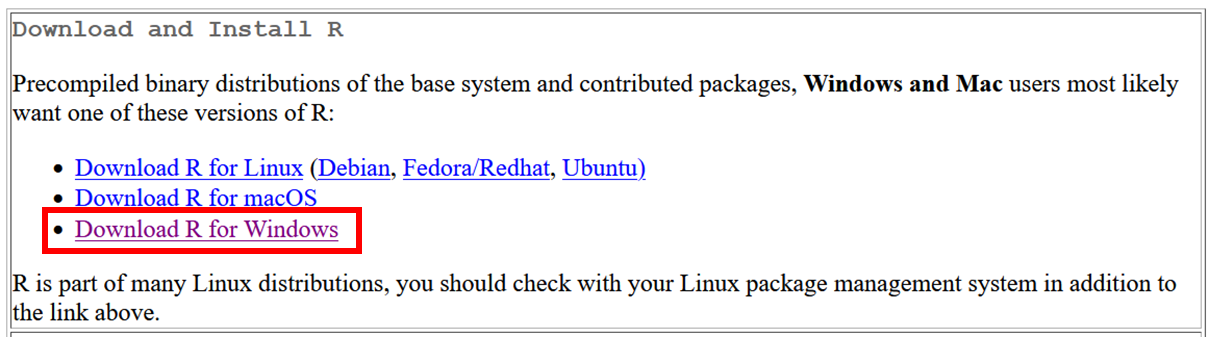
\includegraphics{./images/paste-23A4B16E.png}

\hypertarget{step-3}{%
\subsubsection{Step 3}\label{step-3}}

Select binaries for base distribution

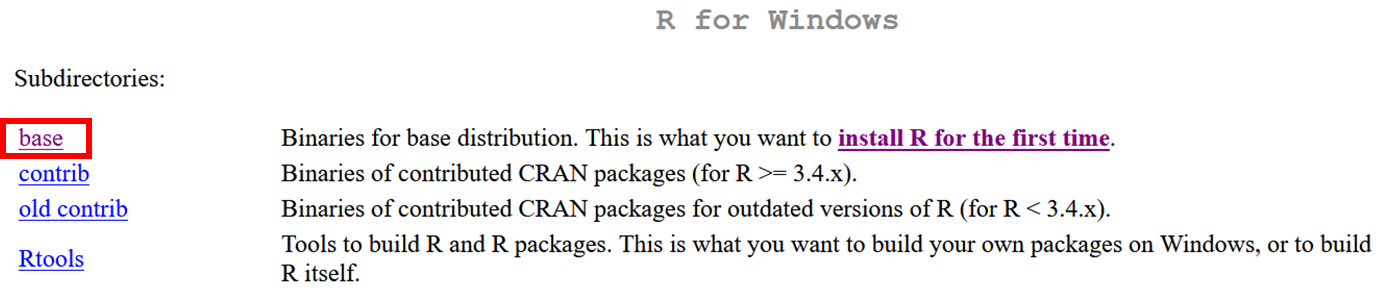
\includegraphics{./images/paste-0739A4C1.png}

\hypertarget{step-4}{%
\subsubsection{Step 4}\label{step-4}}

Download the R installer (\textless{} 80 MB)

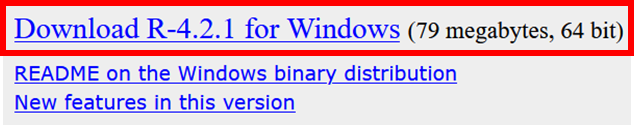
\includegraphics[width=3.64583in,height=\textheight]{./images/paste-9624855F.png}

\hypertarget{step-5}{%
\subsubsection{Step 5}\label{step-5}}

In your computer's Downloads folder, double-click the R setup file.


\includegraphics{./images/paste-FD7C97A4.png}

\hypertarget{step-6}{%
\subsubsection{Step 6}\label{step-6}}

Follow the instruction in the installation wizard to complete the
installation.

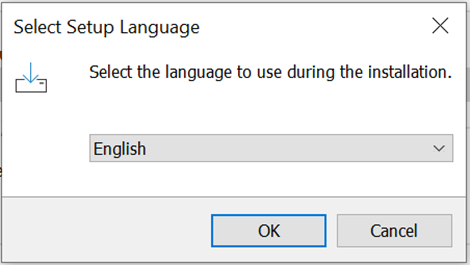
\includegraphics{./images/paste-0F242DBF.png}

\hypertarget{sec-RStudio-installation}{%
\section{Install and setup RStudio
Desktop}\label{sec-RStudio-installation}}

\textbf{Rstudio} is an integrated development environment (IDE) for R
that enables an easier use of R.

\begin{tcolorbox}[enhanced jigsaw, bottomtitle=1mm, title=\textcolor{quarto-callout-note-color}{\faInfo}\hspace{0.5em}{Note}, toptitle=1mm, toprule=.15mm, breakable, colframe=quarto-callout-note-color-frame, coltitle=black, rightrule=.15mm, arc=.35mm, left=2mm, opacitybacktitle=0.6, colback=white, colbacktitle=quarto-callout-note-color!10!white, bottomrule=.15mm, opacityback=0, titlerule=0mm, leftrule=.75mm]
RStudio is moving away from its R-exclusive focus and becoming
\href{https://posit.co/}{Posit} in October 2022 to enable broader data
science, scientific research, and technical communication
functionalities and, in particular, to integrate Python users.
\end{tcolorbox}

\begin{tcolorbox}[enhanced jigsaw, bottomtitle=1mm, title=\textcolor{quarto-callout-important-color}{\faExclamation}\hspace{0.5em}{Important}, toptitle=1mm, toprule=.15mm, breakable, colframe=quarto-callout-important-color-frame, coltitle=black, rightrule=.15mm, arc=.35mm, left=2mm, opacitybacktitle=0.6, colback=white, colbacktitle=quarto-callout-important-color!10!white, bottomrule=.15mm, opacityback=0, titlerule=0mm, leftrule=.75mm]
In order for RStudio desktop to work with R you must have installed R on
your computer, see \textbf{?@sec-R-installation}. RStudio does not
include R when you download and install it.
\end{tcolorbox}

\hypertarget{step-1-1}{%
\subsubsection{Step 1}\label{step-1-1}}

You can download R from the
\href{https://www.rstudio.com/products/rstudio/download/}{RStudio
website}. There are different RStudio products available, but the free
Desktop version offers all necessary features for your analyses.

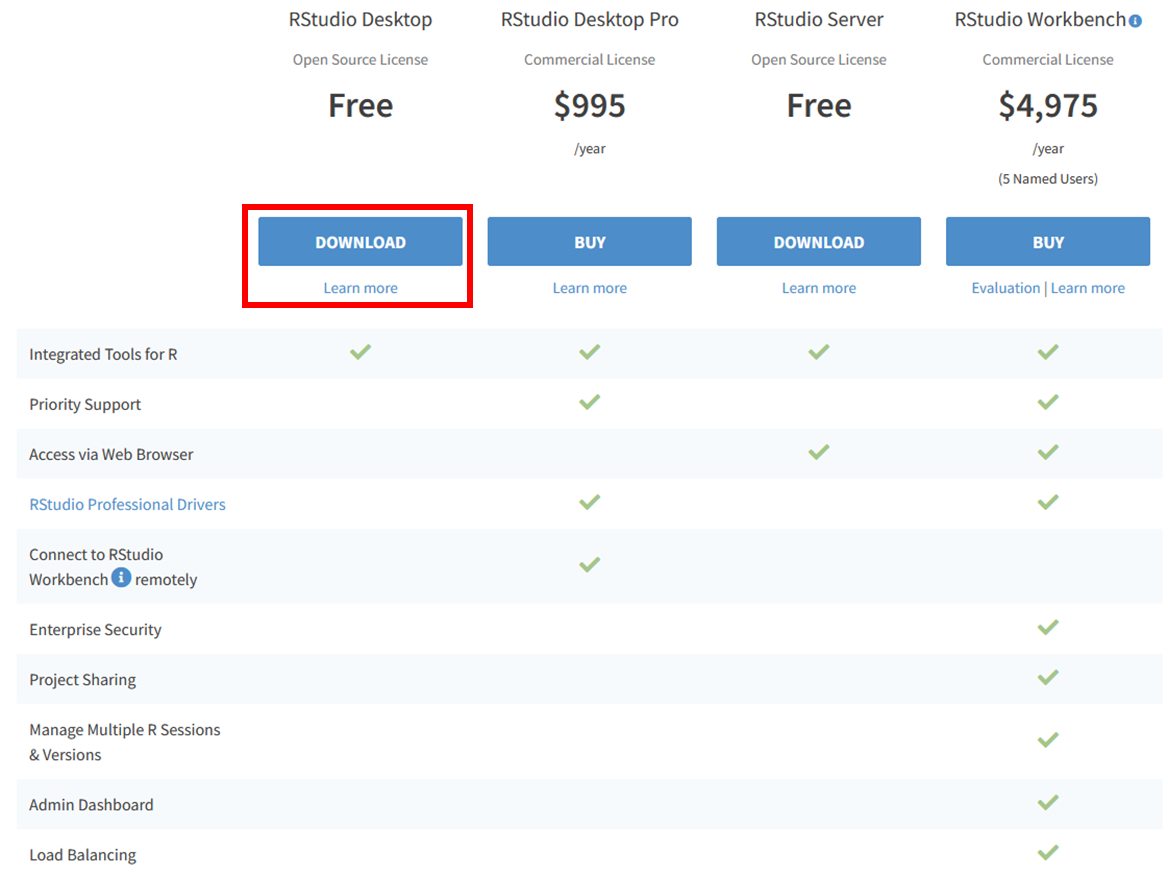
\includegraphics{./images/paste-3C3D0718.png}

\hypertarget{step-2-1}{%
\subsubsection{Step 2}\label{step-2-1}}

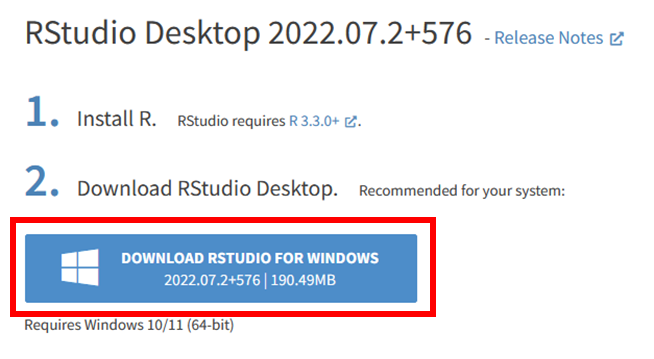
\includegraphics{./images/paste-027BCBD8.png}

Download the RStudio Desktop installer that corresponds to your
operating system.

\hypertarget{step-3-1}{%
\subsubsection{Step 3}\label{step-3-1}}

In your computer's Downloads folder, double-click the RStudio Desktop
setup file.


\includegraphics{./images/paste-31A16011.png}

\hypertarget{step-4-1}{%
\subsubsection{Step 4}\label{step-4-1}}

Follow the instruction in the installation wizard to complete the
installation.

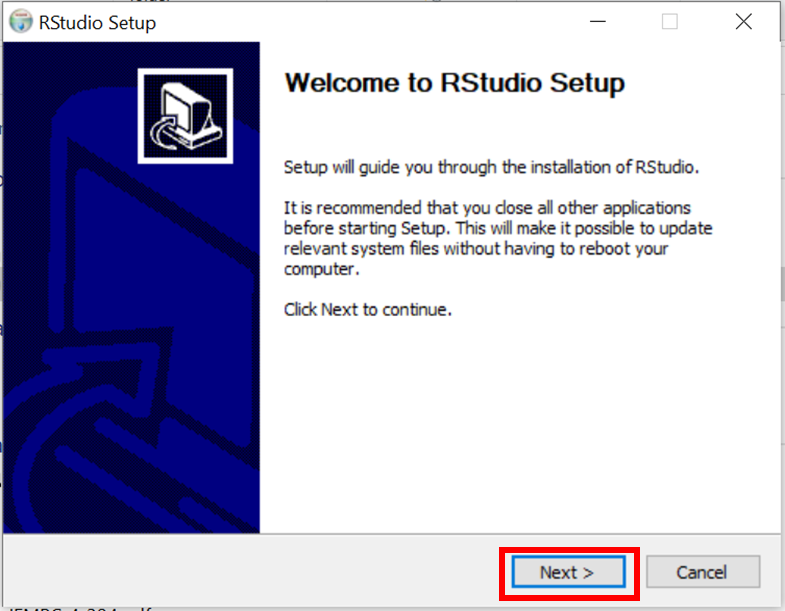
\includegraphics{./images/paste-427EA827.png}

\hypertarget{step-5-1}{%
\subsubsection{Step 5}\label{step-5-1}}

Open RStudio

\hypertarget{step-6-1}{%
\subsubsection{Step 6}\label{step-6-1}}

In RStudio, you can set global options by selecting \textbf{Tools}
\textgreater{} \textbf{Global options}

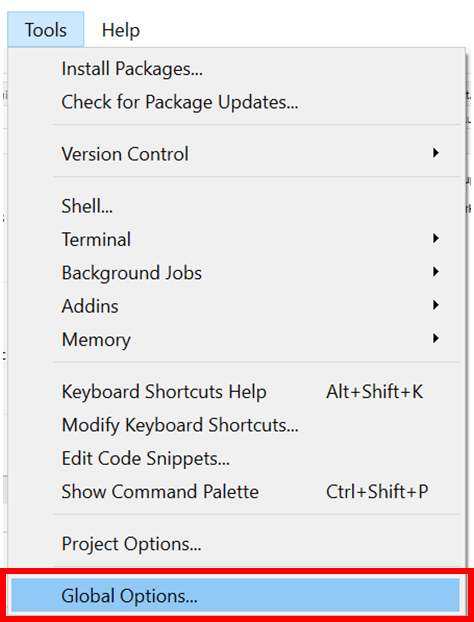
\includegraphics{./images/paste-D0B6CCF0.png}

\hypertarget{step-7}{%
\subsubsection{Step 7}\label{step-7}}

Under the \textbf{General} options and the \textbf{Basic} tab:

\begin{itemize}
\tightlist
\item
  \textbf{Workspace}

  \begin{itemize}
  \item
    Uncheck \emph{Restore .RData into workspace at startup}
  \item
    Ensure that \emph{Never} is selected for \emph{Save workspace to
    .RData on exit}.
  \end{itemize}
\item
  \textbf{History}

  \begin{itemize}
  \item
    Uncheck \emph{Always save history (even when not saving .RData)}
  \item
    Uncheck \emph{Remove duplicate entries in history}
  \end{itemize}
\end{itemize}

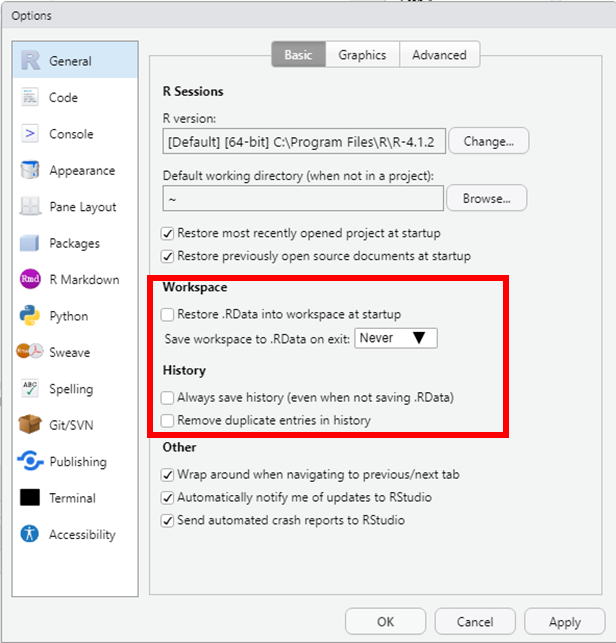
\includegraphics{./images/paste-A507B21D.png}

\hypertarget{sec-Quarto-installation}{%
\section{Install Quarto}\label{sec-Quarto-installation}}

\textbf{Quarto} is a software tool that allows to generate high quality
reproducible data analysis documents (including but not limited to
articles, reports, presentations) with programming language used in data
science (such as R, Python or Julia). It is the successor to \textbf{R
Markdown}.

\hypertarget{step-1-2}{%
\subsubsection{Step 1}\label{step-1-2}}

You can download the Quarto installer that corresponds to your operating
system from the \href{https://quarto.org/docs/get-started/}{Quarto
website}.

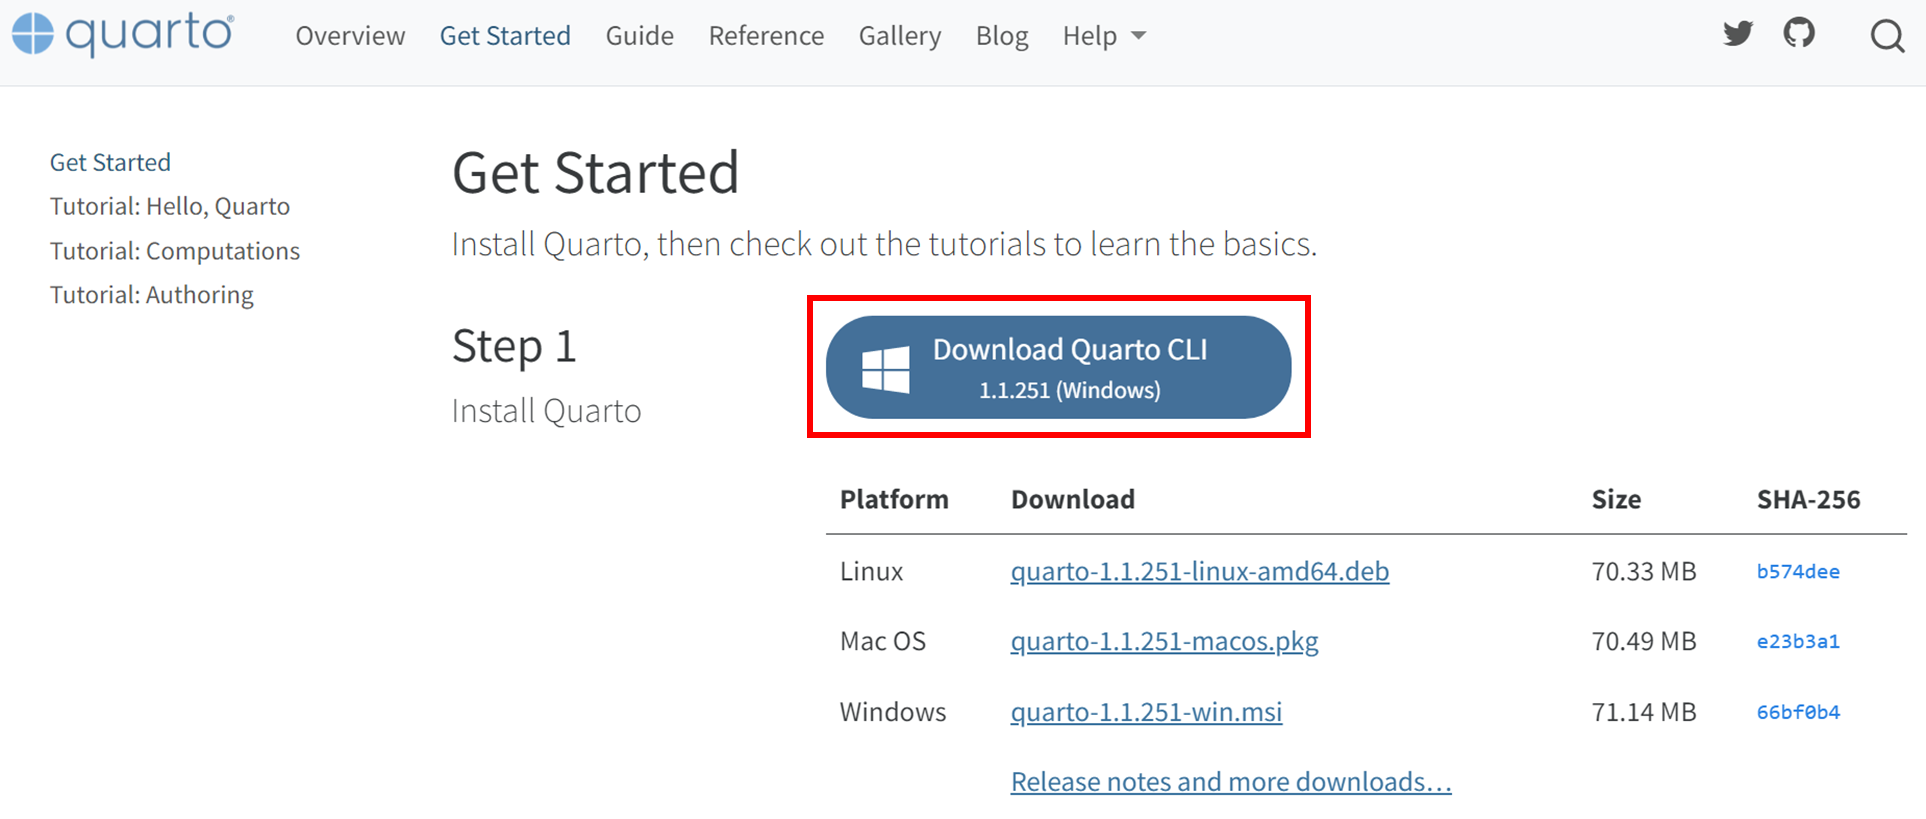
\includegraphics{./images/paste-DDD0332C.png}

\hypertarget{step-2-2}{%
\subsubsection{Step 2}\label{step-2-2}}

1. In your computer's Downloads folder, double-click the Quarto setup
file.

2. Follow the instruction in the installation wizard to complete the
installation.

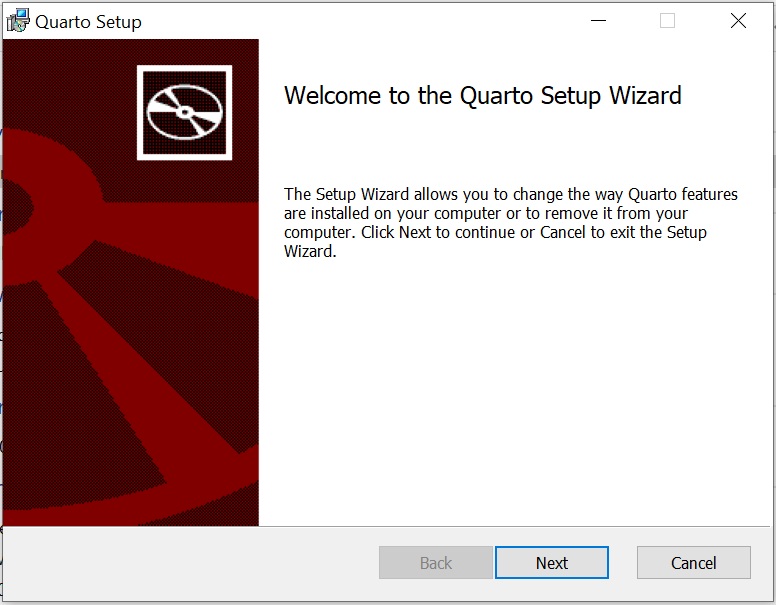
\includegraphics{./images/paste-FE57875E.png}

\begin{tcolorbox}[enhanced jigsaw, bottomtitle=1mm, title=\textcolor{quarto-callout-important-color}{\faExclamation}\hspace{0.5em}{Important}, toptitle=1mm, toprule=.15mm, breakable, colframe=quarto-callout-important-color-frame, coltitle=black, rightrule=.15mm, arc=.35mm, left=2mm, opacitybacktitle=0.6, colback=white, colbacktitle=quarto-callout-important-color!10!white, bottomrule=.15mm, opacityback=0, titlerule=0mm, leftrule=.75mm]
When the installation of Quarto is complete, you will not see any new
software on your computer, but Quarto is now available to be used in
RStudio, as well as by all other applications on your computer.

Quarto will select a version of R by looking on your system PATH. Note
that it is possible to override the version of R used by Quarto by
setting the \texttt{QUARTO\_R} environment variable.
\end{tcolorbox}

\hypertarget{sec-rmarkdown-installation}{%
\section{Install the rmarkdown R
package}\label{sec-rmarkdown-installation}}

To use Quarto with R and RStudio, you need to install the
\textbf{rmarkdown} R package.

\begin{tcolorbox}[enhanced jigsaw, bottomtitle=1mm, title=\textcolor{quarto-callout-note-color}{\faInfo}\hspace{0.5em}{Note}, toptitle=1mm, toprule=.15mm, breakable, colframe=quarto-callout-note-color-frame, coltitle=black, rightrule=.15mm, arc=.35mm, left=2mm, opacitybacktitle=0.6, colback=white, colbacktitle=quarto-callout-note-color!10!white, bottomrule=.15mm, opacityback=0, titlerule=0mm, leftrule=.75mm]
A \textbf{R package} is a collection of functions, data, and compiled
code in a well-defined format, created to add specific functionality to
R.

There are 10,000+ user contributed packages and growing.

There is a set of standard (or base) packages which is considered part
of the R source code and automatically available as part of your R
installation. Base packages contain the basic functions that allow R to
work, and enable standard statistical and graphical functions on data
sets.
\end{tcolorbox}

The \textbf{rmarkdown} package will add all necessary functionalities in
your R installation to render Quarto documents that use R.

\hypertarget{step-1-3}{%
\subsubsection{Step 1}\label{step-1-3}}

Open RStudio on your computer

\hypertarget{step-2-3}{%
\subsubsection{Step 2}\label{step-2-3}}

In RStudio, you can install a new package by selecting \textbf{Tools}
\textgreater{} \textbf{Install packages\ldots{}}

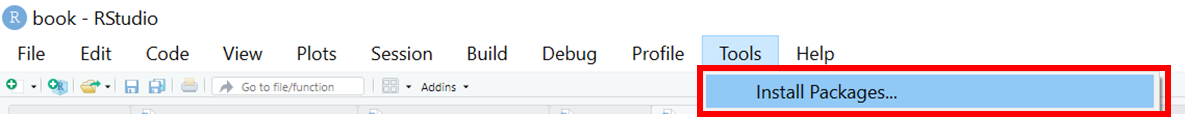
\includegraphics{./images/paste-100922E2.png}

\hypertarget{step-3-2}{%
\subsubsection{Step 3}\label{step-3-2}}

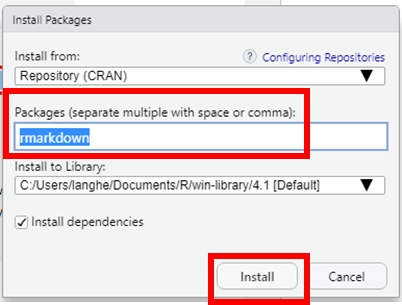
\includegraphics{./images/paste-BE660336.png}

\hypertarget{github-setup}{%
\chapter{GitHub setup}\label{github-setup}}

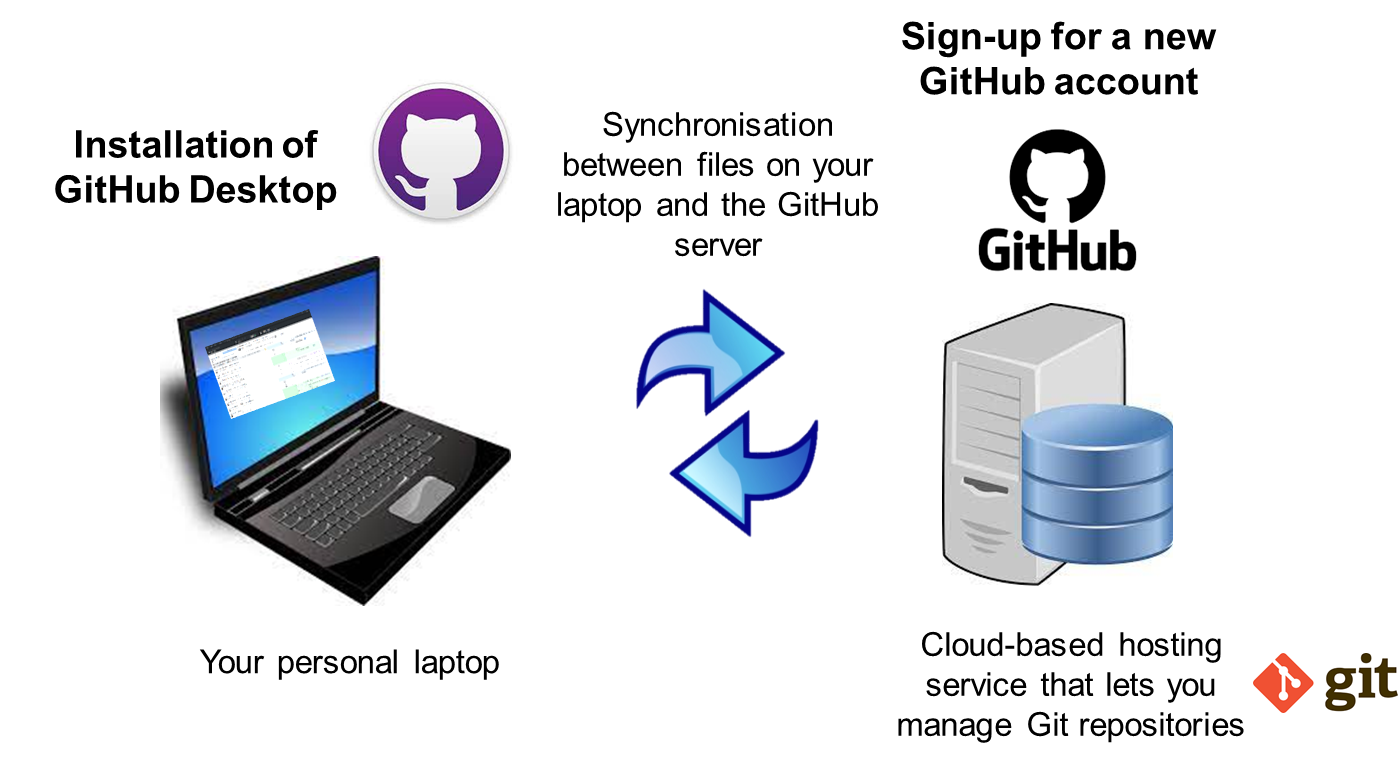
\includegraphics{./images/paste-081F7F03.png}

\textbf{GitHub} is a code hosting platform for version control and
collaboration.

To Create a GitHub account, follow the instructions that are given in
slide 3 of the Powerpoint document available at the following
\href{https://drive.switch.ch/index.php/s/1eFnksrX0UtjfZV}{link}

\hypertarget{sec-GitHub-Desktop-installation}{%
\section{Install GitHub desktop}\label{sec-GitHub-Desktop-installation}}

GitHub Desktop is an application that enables you to interact with
GitHub using an graphical interface instead of the command line or a web
browser.

You can install GitHub Desktop on supported Windows or macOS operating
systems.

\hypertarget{step-1-4}{%
\subsubsection{Step 1}\label{step-1-4}}

\begin{enumerate}
\def\labelenumi{\arabic{enumi}.}
\tightlist
\item
  Visit the \href{https://desktop.github.com/}{download page} for GitHub
  Desktop.
\item
  Click Download for Windows.
\end{enumerate}

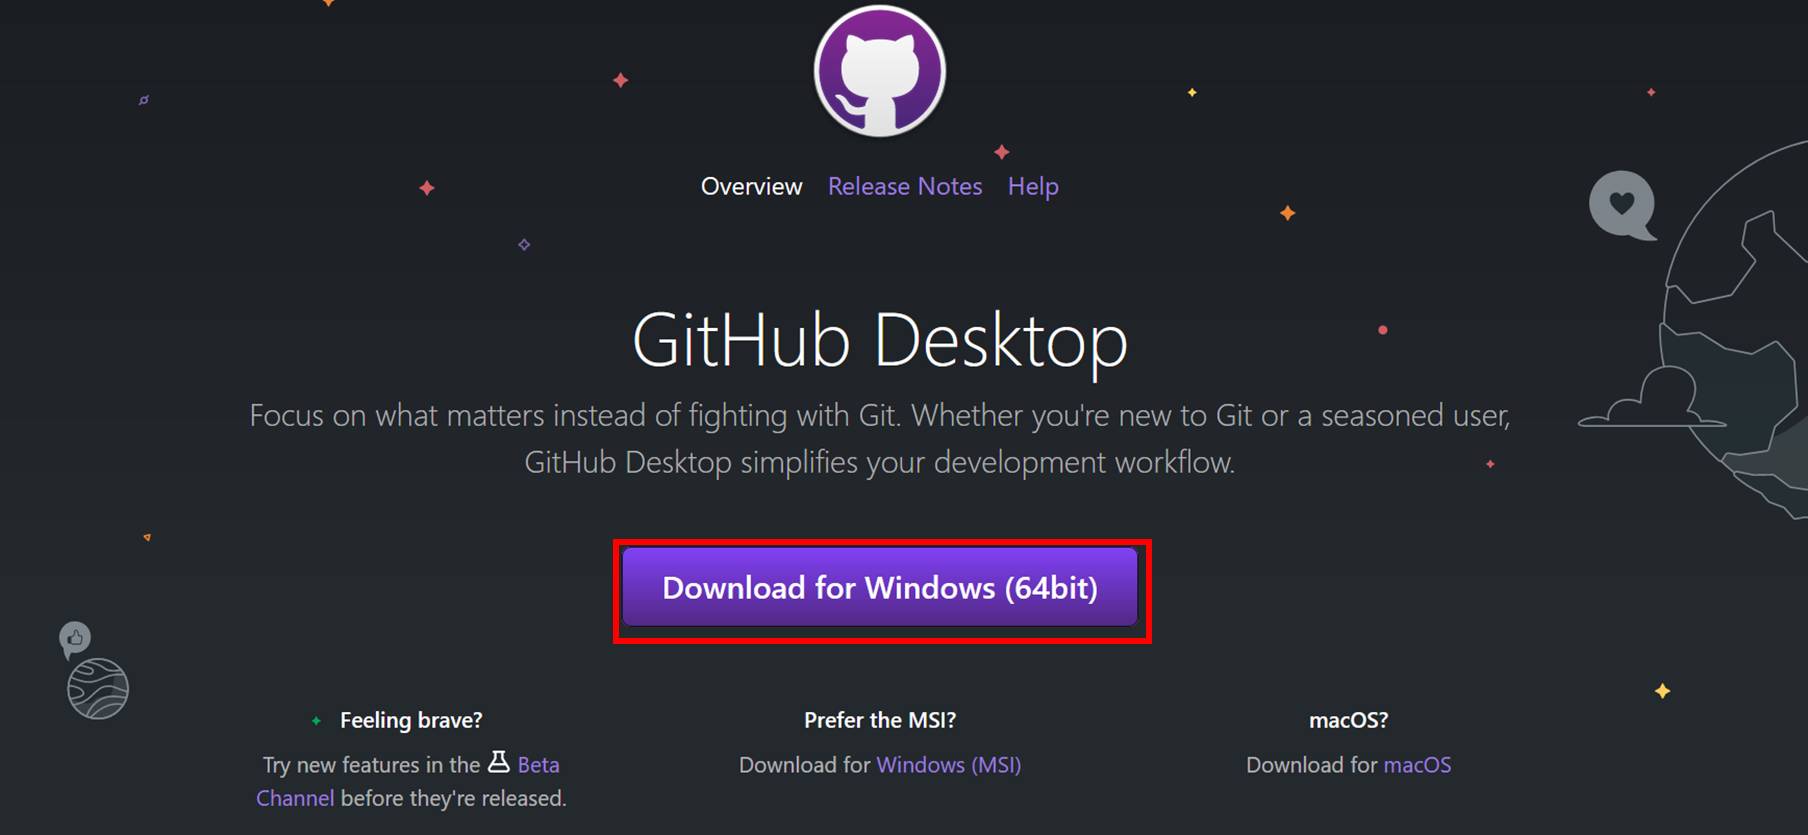
\includegraphics{./images/paste-465BAC3C.png}

\hypertarget{step-2-4}{%
\subsubsection{Step 2}\label{step-2-4}}

\begin{enumerate}
\def\labelenumi{\arabic{enumi}.}
\tightlist
\item
  In your computer's Downloads folder, double-click the GitHub Desktop
  setup file.
\item
  Follow the instruction in the installation wizard to complete the
  installation.
\end{enumerate}

\hypertarget{step-3-3}{%
\subsubsection{Step 3}\label{step-3-3}}

To connect your GitHub account to GitHub Desktop, follow the
instructions that are given in slides 6 to 9 of the Powerpoint document
available at the following
\href{https://drive.switch.ch/index.php/s/1eFnksrX0UtjfZV}{link}



\end{document}
